\documentclass[journal abbreviation, manuscript]{copernicus}

\begin{document}

 %% \ SECTION 2
\section{The phydra package: structure \& features}

- now explain in detail what the package is \& can do, what the structure is like

- clarify that it is situated in complexity between custom scripts and modeling tools with graphical interfaces. It would be possible to design a graphical interface for this later on, but that is not the target audience.

\subsection{Processes}
in xarray-simlab, (almost) everything is a process.
- in the following sections, introduce the specific implementation of xarray-simlab processes within phydra, what is actually implemented in v1 and how it can be modified and used.

\subsubsection{Components}
- Components are state variables, make sure to use clear wording and explain well

\subsubsection{Flows}
- Flows are parts of differential equations, that affect one or more components, and can be influenced by forcing and the physical environment

\subsubsection{Forcing & Physical Environment}
- Forcing can affect one Flow, but can also affect many others, if they are related to the physical environment. This might require a additional fluxes groups defined in the components. 
- explain this here, and present what is included in phydra v1, and how the boilerplate (base classes) can be modified to create your own.

\subsection{Model development workflow}

%%% TWO-COLUMN FIGURES
%
%%f
\begin{figure*}[t]
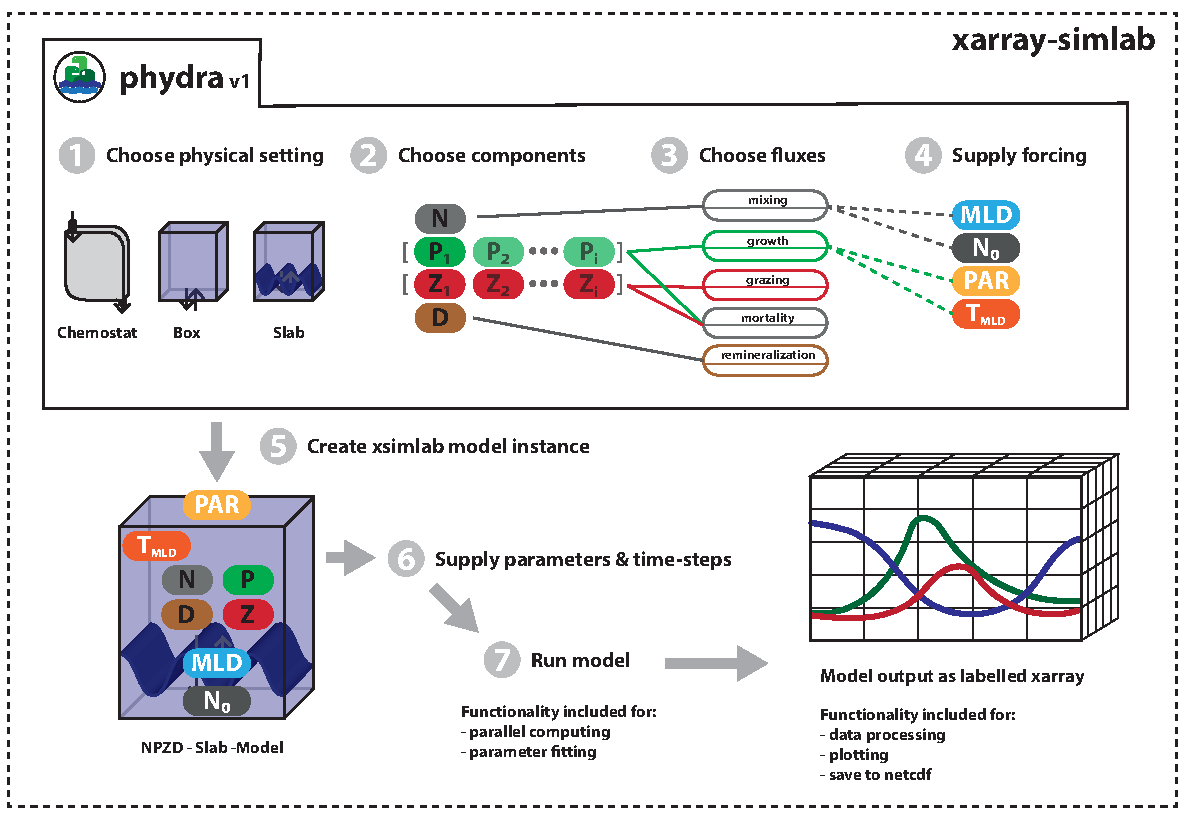
\includegraphics[width=12cm]{Figures/firstdraft_schematics/01__schematics_phydra.pdf}
\caption{Note by Andrew: You will need a much more illuminating figure caption here that describes each step (1, 2, etc) as well as the acronyms/terms (xarray-simlab) and variables (P, Z, D, etc)}
\label{phydraschematics}
\end{figure*}

general explanation, and then go into detail below (see Figure \ref{phydraschematics})

% Everything below here is optional, it depends on what I can actually do in the package
\subsubsection{Dimensionality}
- Dimensionality is a very important fact of building models, and xarray-simlab provides a simple, but sometimes tricky interface for managing dimensionality, so make sure to explain it relatively well here, as well as the implementations.
- I can cite https://www.biogeosciences.net/17/609/2020/ to explain why dimensionality is an important consideration in phytoplankton models.

\subsubsection{Runtime}
- explain what the options are to run the model, depends on if a time implicit method will be added to solve, or if it will just remain with the time explicit steps of xarray-simlab
- mention that xarray-simlab is general enought to support IBMs! But not developed here.

\subsubsection{Model Diagnostics}
- this is a relevant section, *if* Benoît can help me with creating the ODE visualization & model diagnostics.

\subsubsection{Parameter fitting}
- this is a relevant section, if i manage to get some decent parameter fitting results for the example 1 and 3.. either only 3 or both, is my feeling. 

\end{document}